\documentclass[a4paper,11pt]{book}
% Package to make citations superscrit with brackets
\usepackage[super,square]{natbib}
% Package to change margin size
\usepackage{anysize}
\marginsize{1.5cm}{1.5cm}{1cm}{1.5cm} %left/right/top/bottom
% Package to make headers
\usepackage{fancyhdr}
\renewcommand{\headrulewidth}{0pt}
% Package for highlights
\usepackage{soul}
% Colors for the references links
\usepackage[dvipsnames]{xcolor}
% Package to link references
\usepackage{hyperref}
%\usepackage[draft]{graphicx}
\usepackage{graphicx}
\usepackage{float}
\usepackage{physics}
\usepackage{tikz-feynman}
\usepackage{simpler-wick}
\usepackage{tensor}
\usepackage{slashed}
\usepackage{esint}
\usepackage{amsfonts}
\usepackage{mathtools}
\usepackage{amsmath}
\usepackage{amssymb}
\usepackage{amsthm}
\usepackage{enumitem}
\usepackage{setspace} %to set line spacing, see TOC for an example
\usepackage[english]{babel}
\hypersetup{
    colorlinks=true,
    linkcolor=black,
    citecolor=CadetBlue,
    filecolor=CadetBlue,      
    urlcolor=CadetBlue,
}
% Package for lorem ipsum
\usepackage{lipsum}
% Package for multicolumn
\usepackage{multicol}

\usepackage{multicol,caption}
% Package for removing paragraph identations
\usepackage{parskip}
\setlength\columnsep{18pt} 
\setlocalecaption{english}{figure}{Fig.}
\setlocalecaption{english}{table}{Tab.}
\counterwithin{figure}{section} % comandi per numerazione interna di figure, tabelle ed equazioni
\counterwithin{table}{section}
\counterwithin{equation}{section}
\setcounter{tocdepth}{2}
\fancypagestyle{empty}{
    \fancyhead[C]{
	%TESTEMPTY
    }
    \fancyhead[R]{
	%TESTEMPTY
    }
    \fancyhead[L]{
	%TESTEMPTY
    }
    \fancyfoot[C]{
	%TESTEMPTY
    }
    \renewcommand{\headrulewidth}{0.0pt}
}
\fancypagestyle{body}{
    \pagenumbering{arabic}

    \fancyhead[L]{\small{\textbf{Università degli studi di Torino} \\ a.y. 2026/2027}}
    \fancyhead[R]{\small{\textbf{Foundations of QFT notes}\\ Prof. Angelantonj}}
    \fancyfoot[C]{\small{\thepage}}
}


\newcounter{Lessoncounter}
\newcommand\showmycounterL{\addtocounter{Lessoncounter}{1}\themycounter}
\newcommand{\lesson}[1] 
{ {          
    \addtocounter{Lessoncounter}{1}
    \Large \underline{\textbf{Lesson \arabic{Lessoncounter}, #1}}\newline

} 
    %\addcontentsline{toc}{section}{\underline{#1}}    
\addcontentsline{toc}{section}{\underline{\textbf{Lesson \arabic{Lessoncounter}, #1}}}    
}
\newcommand\pd{\partial}
\newcommand{\COMMENT}[1]{} %comment block
% Source - https://tex.stackexchange.com/q/29179
% Posted by PineApple
% Retrieved 2026-11-12, License - CC BY-SA 3.0
%\newcommand{\fdv}[3][]{\frac{\delta^{#1} #2}{\delta #3 ^{#1}}}


 
\begin{document}
\pagestyle{empty}
\begin{center}
\Large{\textbf{Foundations of Quantum Field Theory,\\ Lecture notes}}
\vspace{0.4cm}
\normalsize
\\ Università degli Studi di Torino\\Academic Year 2026/2027 \\Prof. Angelantonj,
notes by Paolo Rocchietti March\footnote{paolo.rocchiettimarc@edu.unito.it} \\

\vspace{0.1cm}
%\textit{Organization}
\medskip
\normalsize
\end{center}
\vspace{0.4cm}
{\color{gray}\hrule}
\tableofcontents
\newpage
\pagestyle{body}

\lesson{09/11}
NO MATERIALS PROVIDED by \textit{choice}, but textbooks (no-one in particular,
but references will be provided).

Two textbooks:
\begin{itemize}
    \item M. Srednicki, \textit{Quantum Field Theory}, Cambridge University Press
        (lots of calculations, less physics);
    \item Iliopoulos, Tomaras, \textit{Elementary Particle Physics}, Oxford
        University Press (NO calculations, lots of physics).
\end{itemize}
In the previous course the classical field theory was quantized with the \textit{
canonical quantization}, in this course Feynman's path (integral) will be taken,
which is a convenient way of computing \textit{correlation functions} (like the
Gell-Man-Low formula), skipping Wick's theorem.
\section{Revision: the Feynman Path Integral Formulation of QM}
This is a revision of some topics covered in the Bachelor's degree course\footnote
{See MQ2 notes, in this same repository} Quantum Mechanics 2.
In QM, the time evolution operator (for a time-independent $H$) is defined as
$$U(t-t_0) = e^{-iH(t-t_0)}$$
where $H=\frac{p^2}{2m}+V(q)$; $U$ has the fundamental property
$$U(t_f-t_i) = U(t_f-t_n)U(t_n-t_{n-1})...U(t_1-t_i)$$
with $t_i<t_1<t_2...<t_n<t_f$.\\
Consider the states $\bra{q_i,t_i}$ and $\bra{q_f,t_f}$:
$$\bra{q_f,t_f} U(t_f-t_i)\ket{q_i,t_i} = \bra{q_f,t_f}U(t_f-t_n)...U(t_1-t_i)
\ket{q_i,t_i}$$
inserting the identities
$$\mathbb{I} = \int_{}^{} \dd q\ket{q}\bra{q}$$
in between the $U$'s yields
$$\int_{}^{} \dd q_n...\dd q_1 = \bra{q_f,t_f}U(t_f-t_n)\ket{q_n,t_n}
\bra{q_n,t_n}...\ket{q_1,t_1}\bra{q_1,t_1}U(t_1-t_i)\ket{q_i,t_i}.$$
Choose now the $t_k$'s so that $\frac{t_f-t_i}{n}=\tau$: all the $U$ become
$$U(\tau)=e^{-iH\tau} = \exp\left[-i(T\tau+V\tau)\right] \underset{\text{BCH}}=
e^{-iT\tau}e^{-iV\tau}e^{-i O(\tau^2)}$$
in the limit $\tau\to 0 \iff n\to\infty$, the $O(\tau^2)$ are negligible, so
$$\bra{q_{j+1},t_{j+1}}U(\tau)\ket{q_j,t_j}\underset{\tau\to0}\sim
\bra{q_{j+1},t_{j+1}}e^{-i\frac{p^2}{2m}\tau}e^{-iV\tau}\ket{q_j,t_j}=
\bra{q_{j+1},t_{j+1}}e^{-i\frac{p^2}{2m}}\ket{q_j,t_j}e^{-iV(q_j)\tau}
$$
because $\hat V\ket{q_j,t_j} = V(q_j)\ket{q_j,t_j}$.\\
To compute the $T$ term, the completeness relation for the $p$ eigenstates
must be inserted
$$\int_{}^{} \dd p_j \bra{q_{j+1},t_{j+1}}e^{-i\frac{p^2\tau}{2m}}\ket{p_j}
\bra{p_j}\ket{q_j,t_j}$$
so, recalling the position-space representation of the $p$ eigenstates,
$$\bra{q_{j+1},t_{j+1}}U(\tau)\ket{q_{j},t_j} = 
\int_{}^{} \dd p_j \exp\left[-i\left(\frac{p_j^2}{2m}+V(q_j)\right)+
ip_j(q_{j+1}-q_j)\right].$$
So the full expression is
$$\bra{q_i,t_i}U(t_f-t_i)\ket{q_f,t_f} =
\prod_{j=1}^{n}\int_{}^{} \dd q_j\dd p_j \exp\left[-i\left(\sum_{j=1}^{n}
\frac{p_j^2}{2m}+V(q_j)\right)\tau + ip_j\tau\frac{q_{j+1}-q_j}{\tau}\right]
$$
making this relation continuous yields

$$\bra{q_i,t_i}U(t_f-t_i)\ket{q_f,t_f} = 
\int \left(\prod_{j}^{}\dd q_j\dd p_j\right)\exp\left[-i
\int_{t_i}^{t_f} \dd t \left(\frac{p^2}{2m}+V(q)\right) - p\dot q \right]
$$
completing the square in the exponent and adding $\hbar$ yields
$$\bra{q_i,t_i}U(t_f-t_i)\ket{q_f,t_f} = \int \mathcal{D}q \exp\left[
\frac{i}{\hbar} \int_{t_i}^{t_f} \dd t
\underbrace{\left(\frac{m}{2}\dot q^2 -V(q)\right)}_{:=\mathcal{L}}\right]$$
The kind of integral in the exponent are difficult to compute directly with
$\hbar\to0$: one can use the \textit{saddle point technique}.

Suppose to find the transition amplitude of $q(\tilde t)$ (position operator!)
$$\bra{q_f,t_f}q(\tilde t)\ket{q_i,t_i} = \bra{q_f,t_f}U(t_i-\tilde t)q(t)U(
\tilde t-t_f)\ket{q_i,t_i}:$$
the aforementioned process can be here used by evaluating $\hat q\ket{q_k,t_k} = 
q(t_k)\ket{q_k,t_k}$ (with $t_k$ close to $\tilde t$) and yields
$$\bra{q_f,t_f}q(\tilde t)\ket{q_i,t_i}=\int_{}^{} \mathcal{D}q e^{
\frac{i}{\hbar}S}q(\tilde t).$$
And with a time ordered product?
$$\bra{q_f,t_f}T\left(q(t_a)q(t_b)\right)\ket{q_i,t_i}$$
without loss of generality, assume $t_a>t_b$:
$$\bra{q_f,t_f}T\left(q(t_a)q(t_b)\right)\ket{q_i,t_i}$$
now the process will be repeated with $t_k$ close to $t_a$ and $t_j$ close to
$t_b$ and in the end
$$\bra{q_f,t_f}T\left(q(t_a)q(t_b)\right)\ket{q_i,t_i}=\int \mathcal{D}q
e^{\frac{i}{\hbar}S}q(t_a)q(t_b)$$
On the other hand, if $t_b>t_a$, the result is the exact same! 

$$\int \mathcal{D}q e^{iS} q(t_1)...q(t_n) = \bra{q_i,t_i} T\left\{q(t_1)...q(t_n)
\right\}\ket{q_f,t_f}$$

The measure of integration $\mathcal{D}q$ is not mathematically well defined, but
it can be interpreted as the integration over all \textit{paths} that
link the initial and final position.

[smth like $\bra{a}...\ket{b} = \int...$]

This can also be generalized to $t_i=-\infty$, $t_f=\infty$: consider the state
$$\ket{q_i,t_i}=e^{-iHt_i}\ket{q_i}=\sum_{n}^{}e^{-iHt_i}\ket{n}\bra{n}\ket{q_i}$$
Suppose $E_0=0$ (or change $H$ so that it is) and ``suppose $t$ is slightly
imaginary'' and goes to $-\infty$ i.e $t\to -\infty(1+i\varepsilon)$: the
$n\neq0$ states' contributions are negligible (because the exponential
has a real part multiplied by $-\varepsilon $)
and similarly for the $\ket{q_f}$ eigenstate: this means that only the vacuum
state matters, i.e.
$$\int \mathcal{D}q e^{iS} q(t_1)...q(t_n) = \bra{0}T\left\{q(t_1)...q(t_n)
\right\}\ket{0},\; t_i,t_f\to\pm\infty$$
\subsection{Gaussian Integrals}
Suppose to evaluate the $n$-th statistical momentum of the Gaussian
$$M_n=\int_{-\infty}^{\infty} \dd x e^{-Ax^2}x^n$$
one can use the Euler $\Gamma$ function by letting $x^2=t$, or consider
\[
    I(t) = \int_{-\infty}^{\infty} \dd x e^{-Ax^2-tx},
\]
since it is clear that
\[
    M_n =\eval{(-1)^n \dv[n]{}{t}I(t)}_{t=0}:=\eval{\left(-\dv[]{}{t}\right)^n
    I(t)}_{t=0}.
\]
This integral can be explicitely computed:
\begin{gather*}
    I(t) = \int_{-\infty}^{\infty} \dd x e^{-Ax^2-tx} = \int_{}^{} \dd x
    \exp\left[-A\left(x^2+\frac{t}{A}x+\left(\frac{t}{2A}
    \right)^2\right) + A\left(\frac{t}{2A}\right)^2\right] =\\= 
    e^{A\left(\frac{t}{2A}\right)^2}\int_{-\infty}^{\infty} \dd xe^{\left(
    x+\frac{t}{2A}\right)^2}= e^{A\left(\frac{t}{2A}\right)^2}\sqrt{\pi}
\end{gather*}
$I(t)$ is called the \textit{generator function of the n-th order momentum of
the Gaussian}, since, by construction,
$$I(t) = \sum_{n=0}^{\infty}M_n\frac{(-t)^n}{n!}.$$


\lesson{10/11}
The generator function is defined with a normalization:
$$I(t) = \frac{\int_{-\infty}^{\infty} \dd x \exp\left[ -Ax^2-tx \right]}{
\int_{-\infty}^{\infty} \dd x e^{-Ax^2}}$$
and it can be expanded in Taylor Series as
$$I(t)= \sum_{n=0}^{\infty}M_n(A)\frac{(-t)^n}{n!},\quad
M_n=\eval{\left(-\pdv{}{t}\right)^n I(t)}_{t=0}$$
and $M_n$ is the $n-$th statistical moment of the Gaussian distribution.

Integrals like the numerator of $I(t)$ can be computed by completing the
square:
$$I(t) = \frac{\int_{-\infty}^{\infty} \dd x \exp\left[ -A(x+\flatfrac{t}{2A})^2
+\flatfrac{t^2}{4A}\right]}{\int_{-\infty}^{\infty} \dd x e^{-Ax^2}} = 
e^{\flatfrac{t^2}{4A}}
$$
And from this follow the momenta of the Gaussian and the fact that the odd momenta
are zero, since every odd derivative of $I(t)$ is proportional to $t$ and
vanishes.

\textbf{Example} $M_4$
\[
    M_4 = \eval{\pdv[4]{}{t}I(t)}_{t=0} = \eval{\pdv[2]{}{t}M_2(t)}_{t=0}=
    [...] = \frac{3}{4A^2}
\]

Another kind of Gaussian integral is
\[
I=\int_{-\infty}^{\infty} \dd x \exp\left[ -Ax^2 +f(x) \right]
\]
the first step is to expand $e^{f(x)}=g(x)$ around $x=0$:
\[
    e^{f(x)} = \sum_{n=0}^{\infty}c_nx^n
\]
so
\[
    I=\sum_{n=0}^{\infty}c_n\int_{-\infty}^{\infty} \dd x e^{-Ax^2}x^n
\]
but the integral is now the (non-normalized) $n-$th Gaussian momentum:
\[
    I=\frac{1}{\sqrt{\pi}}\sum_{n=0}^{\infty}c_n \eval{\left(-\dv[]{}{t}\right)^n
    \int_{-\infty}^{\infty} \dd x e^{-Ax^2-tx}}_{t=0}
\]
formally, the series is the Taylor expansion of $g\left(-\pdv[]{}{t}\right)$:
\[
    I = \frac{1}{\sqrt{\pi}}\eval{e^{f\left(-\pdv[]{}{t}\right)} I(t)}_{t=0}
\]
where
\[
    I(t) = e^{\frac{t^2}{4A}}.
\]
This expression is complicated, but it is useful in a perturbative framework,
since if $f=\alpha f$ and $\alpha$ is a small, dimensionless parameter, the
integral is approximated, ignoring normalizations, as
\[
I(t)=f\left(-\dv[]{}{t}\right)I(t) + \frac{\alpha^2}{2!} f^2\left(-\dv{}{t}
\right)I(t)+O(\alpha^3)
\]

\chapter{Path Integral Quantization for QFT}
\section{Introduction}
This new quantization technique for QM computes the Green function of the
Schrödinger operator as follows:
\[
    Z = \int \mathcal{D}q e^{iS},\;\text{with } S=\int_{}^{} \dd t \left(
    \frac{m}{2}\dot q^2-V(q)\right)
\]
The equivalent expression for the scalar field uses
\[
    \mathcal{L} = \frac{1}{2}\pd_\mu\phi\pd^\mu\phi - \frac{1}{2}m^2\phi^2
\]
and so the expectation value of the time-ordered product of fields is
\[
    \bra{0}T\left\{\phi(x_1)...\phi(x_n)\right\}\ket{0} =
    \int \mathcal{D}\phi e^{iS} \phi(x_1)...\phi(x_n)
\]
A convenient way to compute this kind of integral is to use this
\[
    Z[J]=\int \mathcal{D}\phi \exp\left[ iS + i\int_{}^{} \dd^4x J(x)\phi(x)
    \right] 
\]
the integral at exponent is a \textit{source term}, since
\[
S+\int_{}^{} \dd^4x J(x)\phi(x) = \int\dd^4\left(\mathcal{L}_s+J(x)\phi(x)\right)
\]
and the corresponding Euler-Lagrange equation is
\[
\pd_\mu\left(\frac{\delta\mathcal{L}}{\delta\pd_\mu\phi}-
\pdv{\mathcal{L}}{\phi}\right) = 0 \iff \Box\phi +m^2\phi -J = 0 \iff
\boxed{\left(\Box+m^2\right)\phi = J}
\]
which is similar to a wave equation with a source.

Another notation is
\[
    \langle A \rangle_{x,y,z...} := \int_{}^{} \dd^4x\dd^4y\dd^4z... A
\]
Since this $J$ term is just a computation trick, another concept is useful
to use it: the functional derivative of a field with respect to itself is
\[
\frac{\delta}{\delta \phi(x)}\phi(y):=\delta^4(x-y)
\]
So
\[\eval{-i\frac{\delta}{\delta J(y)} Z[J] }_{J=0}=\eval{ \int \mathcal{D}\phi -i
\frac{\delta}{\delta J(y)}\left(e^{i\langle\phi J\rangle}\right)e^{iS}}_{J=0}=
\eval{\int \mathcal{D}\phi \phi(y)e^{iS + i\langle\phi J\rangle}}_{J=0}=
\int \mathcal{D}\phi\phi(y)e^{iS}
\]
So to bring down bigger powers of $\phi$ into the integrand, more derivatives
are required, so
\[
\bra{0}T\left\{\phi(x_1)...\phi(x_n)\right\}\ket{0} = 
\eval{\prod_{i=1}^{n} \left(-i\frac{\delta}{\delta J(x_i)}\right) Z[J]}_{J=0}
\]
So, in parallelism with the Gaussian integrals, $\mathbf{J(x)}$ \textbf{is the
generating function} of the Green functions (i.e. the vacuum-expectation
value of time ordered product of fields, i.e. Feynman propagators), since
\[
    Z[J]=\sum_{n=0}^{\infty}G_n(x_1,...x_n)\frac{1}{n!}\prod_{i=i}^{n}J(x_i)
\]

\section{Free theory}
Consider the free action $S_0$:
\[
    Z_0[J] = \int \mathcal{D}\phi e^{iS_0+i\langle J\phi\rangle_x}
\]
the exponent is
\[
    S_0 + \langle J\phi\rangle = \int_{}^{} \dd^4x \left[\frac{1}{2}\pd_\mu\phi
    \pd^\mu\phi - \frac{m^2}{2}\phi^2+J\phi\right]
\]
Here the square that must be completed is the $\phi^2$ term: the difficult thing
are the differential operators, so consider the F.Ts of $\phi$ and $J$:
\[
    \phi(x)=\frac{1}{(2\pi)^4}\int_{}^{} \dd ^4k e^{ikx}\tilde\phi(k),\quad 
    J(x)=\frac{1}{(2\pi)^4}\int_{}^{} \dd^4k e^{ikx}\tilde J(k)
\]
and plug them in
\[
S_0+\langle J\phi\rangle_x = \int_{}^{} \dd^4x\frac{\dd^4k\dd^4\tilde k}{
(2\pi)^8}\left(-\frac{1}{2}k\tilde k\tilde\phi(k)\tilde \phi(\tilde k) -
\frac{m^2}{2}\tilde\phi(k)\tilde\phi(\tilde k)+\frac{1}{2}\left(
\tilde J(k)\tilde\phi(\tilde k) + \tilde J(\tilde k)\tilde \phi(k)\right)\right)
e^{i(k+\tilde k)x}
\]
With the exponential and a $(2\pi)^4$ factor a $\delta^4(k+\tilde k)$ can be
constructed:
\[
S_0+\langle J\phi\rangle_x = \frac{1}{2}\int_{}^{} \frac{\dd^4k}{(2\pi)^4}
\left(
\left(k^2-m^2\right)\tilde\phi(-k)\tilde\phi(k) +\tilde J(-k)\tilde\phi(k)+
\tilde\phi(-k)\tilde J(k)
\right)
\]
Adding 
\[
0 = (k^2-m^2)\frac{\tilde J(k)\tilde J(-k)}{(k^2-m^2)^2}-
\frac{\tilde J(k)\tilde J(-k)}{k^2-m^2}
\]
``completes the square'', yielding
\[
S_0 + \langle J\phi\rangle_x = 
\frac{1}{2}\int_{}^{} \frac{\dd^4k}{(2\pi)^4}
\left\{
\left[\tilde \phi(-k)+\tilde J(-k)\frac{1}{k^2-m^2}\right](k^2-m^2)
\left[\tilde \phi(k)+\tilde J(k)\frac{1}{k^2-m^2}\right] - \tilde J(-k)\frac{1}{
k^2-m^2}\tilde J(k)
\right\}
\]
by defining
\[
\tilde \varphi(k) = \tilde \phi(k) + \tilde J(k)\frac{1}{k^2-m^2}
\]
the measure of the functional integral does not change and the exponent is
\[
S_0+\langle J\phi\rangle_x = 
\frac{1}{2}\int_{}^{} \frac{\dd^4k}{(2\pi)^4}
\left\{
\tilde \varphi(-k)(k^2-m^2)\tilde\phi(k)-\tilde J(-k)\frac{1}{k^2-m^2}\tilde J(k)
\right\}
\]
So the $Z_0$ is
\[
    Z_0[J] = \int \mathcal{D}\varphi \exp\left[ \frac{i}{2}
    \int_{}^{} \frac{\dd^4k}{(2\pi)^4}\tilde \varphi(-k)(k^2-m^2)\tilde\varphi(k)
\right]\exp\left[ -\frac{i}{2}\int_{}^{} \frac{\dd^4k}{(2\pi)^4}
\tilde J(-k)\frac{1}{k^2-m^2}\tilde J(k) \right]
\]
antitransforming
\[
    \tilde\varphi(k)=\int_{}^{} \dd ^4x e^{-ikx}\varphi(x),\quad
    \tilde J(k) = \int_{}^{} \dd ^4x e^{-ikx} J(x)
\]
Plugging these in and observing
\[
    k^2 e^{-ik(x-y)}=\pdv{}{x_\mu}\pdv{}{y^\mu}e^{-ik(x-y)}
\]
the $\varphi(x)(k^2-m^2)\varphi(y)$ term can be integrated by parts and yields
the original action
\[
    \int_{}^{} \frac{\dd^4k}{(2\pi)^4}e^{-ik(x-y)}\int\dd^4x\int\dd^4y
\left(\pd_\mu\varphi(x)\pd^\mu\varphi(y) - m^2\varphi(x)\varphi(y)\right)=
S_0
\]
So, redefining $Z_0[J]$ \textit{without} this normalization
\[
    Z_0[J] = \frac{\int \mathcal{D}\phi e^{iS_0+i\langle J\phi\rangle_x}}{
        \int \mathcal{D}\phi e^{iS_0}
    }=
    \exp\left\{ -\frac{i}{2}\int \dd^4x\int\dd^4y J(x)
    \underbrace{\int\frac{\dd^4k}{(2\pi)^4}
    \frac{e^{-ik(x-y)}}{k^2-m^2}}_{:=-i\Delta_F(x-y)}J(y)\right\}
\]
So finally
\[
\boxed{Z_0[J]=\exp\left[-\frac{1}{2}\langle J(x)\Delta(x-y)J(y)\rangle_{xy}
\right]}
\]
\textbf{Note} These are not properly Gaussian integrals, since $e^{ix^2}$ does not
converge, but this can be solved by giving a little imaginary part to the mass
$m\to m-i\varepsilon$, which brings the $+i\varepsilon$ to the denominator of the
propagator.

Another way to solve this is by using a \textbf{Wick Rotation}
\[
t\to\tau:=\pm it
\]
which makes the Minkowski metric \textit{euclidean}: in this context using the
mostly positive metric is better, since the resulting metric tensor is exactly
the euclidean one and not its opposite. This can be used as follows (+,-,-,-)
\[
i\int\dd^4x\frac{1}{2}\left(\pd_\mu\phi\pd^\mu\phi - \frac{m^2}{2}\phi^2\right)=
i(\mp i)\int_{}^{} \dd^4x_e\frac{1}{2}\left(-\pd_\mu\phi\pd_\nu\phi
\delta^{\mu\nu}+m^2\phi^2\right) = \mp\int\dd^4x_e\frac{1}{2}\left(\pd_\mu\pd_\nu
\delta^{\mu\nu}+m^2\phi^2\right)
\]
The sign suggests to choose the $+$ sign in Wick's rotation.
\[
\tau=it,\quad iS_0:=-S_e
\]
and the euclidean partition function is
\[
    Z_0^e[J]=\int \mathcal{D}\phi \exp\left[ -S_e -\langle J\phi\rangle_x \right]
\]


\lesson{11/11}



\[
    Z_0[J] = \sum_{n=0}^{\infty} \frac{i^N}{N!}\langle 
    G(1,2...N)J_1...J_N    \rangle_{1...N}
\]
And so the Green function, as seen before, is
\[
    G(1...N) = \eval{(-i)^N\frac{\delta^N}{\delta J_1...\delta J_N}Z_0[J]
}_{J_i=0}\]
\textbf{Explicit examples}\\
\[
    G_1(x_1)=\eval{-i\frac{\delta }{\delta J_1} Z_0[J] }_{J=0}= \eval{(-i)\left(-
    \frac{1}{2}\right)\frac{\delta }{\delta J_1}\left(\langle J(x)\Delta (x-y)
    J(y)\rangle_{xy}\right)Z_0[J]
}_{J=0}\]
the functional derivative acts on the exponent, yielding
\[
    G_1(x_1) = \eval{i \langle \underbrace{\frac{\delta J(x)}{\delta J(x_1)}}_{=
    \delta^4(x-x_1)}\Delta (x-y)J(y)\rangle_{xy}Z_0[J]}_{J=0}=
    \eval{i\langle \Delta (x_1-y)J(y)\rangle_yZ_0[J]}_{J=0}=0
\]

If there are two fields
\begin{gather*}
    G_2(x_1,x_2) = \eval{-\frac{\delta^2}{\delta J_1\delta J_2}}_{J=0}=
    \eval{\frac{\delta }{\delta J_2}\left(\langle \Delta (x-y)J(y)\rangle_y Z_0[J]
    \right)}_{J=0}=\\=
    \eval{-\Delta (x_1-x_2 )Z_0[J] - \langle \Delta (x_1-y)J(y)\rangle_y\underbrace{
    \frac{\delta }{\delta J_2}Z_0[J]}_\text{prev. res.}}_{J=0}=\\=
    \eval{-\Delta (x_1-x_2 )Z_0[J] + \langle \Delta (x_1-y)J(y)\rangle_y
    +\langle \Delta (x_2-w)J(w)\rangle_w Z_0[J]}_{J=0}=\\=-\Delta (x_1-x_2)
\end{gather*}
The $G_3$ propagator is again null, since an odd number of derivatives brings down
$J$ terms that vanish when setting $J=0$ (much like the Gaussian integrals).

For $4$ fields,
\begin{gather*}
    \eval{G_4 = \frac{\delta ^4}{\delta J_1\delta J_2\delta J_3}Z_0[J]}_{J=0}=
    \eval{\frac{\delta ^3}{\delta J_1\delta J_2\delta J_3}\left(
    \langle -\Delta (x_4-y)J(y)\rangle_y Z_0[J]
    \right)}_{J=0}=\\
    =\frac{\delta^2}{\delta J_1\delta J_2}\eval{\left(
    \left(-\Delta_{4,3}+\langle \Delta_{4,y}J_y\rangle_y\langle \Delta_{3w}J(w)
    \rangle_W\right)Z_0[J]\right)}_{J=0} = \\
    =\eval{\frac{\delta }{\delta J_1}\left(\left(
    \Delta_{43}\langle \Delta_{2y}J(y)\rangle_y + \Delta_{42}\langle \Delta_{3w}
    J(w)\rangle_w + \langle \Delta_{4y}J(y)\rangle_y\Delta_{32}-
    \langle\Delta_{4y}J(y)\rangle_y\langle \Delta_{3w}J(w)\rangle_w\langle 
    \Delta_{2z}J(z)\rangle_z\right)Z_0[J]\right)}_{J=0}=\\
    =\footnote{mi son perso...}
    \Delta_{32}\Delta _{41}-\Delta _{32}\langle \Delta _{4y}J_y\rangle_y
    \langle \Delta_{1w}J_w\rangle_w [... termini]
\end{gather*}
these are all possible derivatives of $4$-th order, by setting $J=0$, all the
$\langle ...J\rangle_{i}\Delta_{kj}$ will vanish, so
\[
G_4 = \Delta_{43}\Delta_{21} + \Delta_{42}\Delta_{31}+\Delta_{41}\Delta_{32}
\]
A trick to take these derivatives is to only compute those that will result in
terms independent of $J$!.

The result is known! These are the contractions seen in IQFT!
\[
    G_4 = \bra{0}T\left\{\phi _1\phi _2\phi _3\phi _4\right\}\ket{0} = 
    \bra{0} N\left\{\phi _1...\phi _4 + \text{contractions}\right\}\ket{0}=
    \bra{0}\overline{\phi_1\phi _2}\,\overline{\phi_3\phi _4} + ...\ket{0}
\]
and the result is the same!! This means that Wick's theorem is built-in for the
path integral formulation.

Is there a formal way to exclude non-connected Feynman Diagrams?

Consider
\[
    Z_0[J]= e^{-W_0[J]}
\]
where $W_0[J]$ is called the \textit{Free energy operator}; so
\[
    W_0[J] = \frac{1}{2}\int_{}^{} \dd ^4x\dd^4y J(x)\Delta(x-y)J(y)
\]
This generates \textbf{only connected Feynman diagrams}:
\[
W_0[J]=\sum_{N=0}^{\infty} \frac{1}{N!}\langle J_1...J_NG^C(1...N)\rangle_{1..N}
\implies \eval{G^C(1...N)=\frac{\delta^N}{\delta J_1...\delta J_N}W_0[J]}_{J=0}
\]
for the free theory this is due to the fact that $W_0$ is quadratic in $J$ and
all higher or lower order derivatives are null.

\section{Interacting theories: introduction}
The interacting action is
\[
    S=\int_{}^{} \dd ^4x\left(\frac{1}{2}\pd_\mu\phi \pd^\mu\phi -\frac{m^2}{2}
    \phi^2 -V(\phi)\right) = S_0 - \int_{}^{} \dd ^4x V(\phi)
\]
The partition function for interacting theories is
\begin{gather*}
    Z[J]=\frac{\int \mathcal{D}\phi
    \exp\left[iS+i\langle J\phi \rangle_x\right]}
    {\int \mathcal{D}\phi e^{iS_0}} = 
    \frac{\int \mathcal{D}\phi
    \exp\left[ -i\int_{}^{} \dd^4x V(\phi) \right]
    \exp\left[iS_0+i\langle J\phi \rangle_x\right]}
    {\int \mathcal{D}\phi e^{iS_0}} = \\
    =\mathcal{N} \int \mathcal{D}\phi e^{-i\langle V\rangle}e^{iS_0+i\langle 
    \phi J\rangle}
\end{gather*}
considering
\[
    e^{-i\langle V\rangle }=\sum_{n}^{} c_n\phi^n 
\]
this becomes, much like the gaussian integrals,
\begin{gather*}
    Z[J]=\mathcal{N}\sum_{n}^{} c_n \int \mathcal{D}\phi \phi^ne^{iS_0+i\langle
    \phi J\rangle } = \mathcal{N}\sum_{n}^{} c_n\int \mathcal{D}\phi \left(
    -i\frac{\delta}{\delta J}\right)^ne^{iS_0+\langle \phi J\rangle }=\\
    =\exp\left[ -i\langle V\left(-i\frac{\delta }{\delta J}\right)
    \rangle_x\right]\underbrace{\frac{\int \mathcal{D}\phi \exp\left[ iS_0
    +i\langle J\phi\rangle_x  \right]}{\int \mathcal{D}\phi e^{iS_0}}}_{:=Z_0[J]}=
    \\=\exp\left[ -i\langle V\left(-i\frac{\delta }{\delta J}\right)
    \rangle_x\right] Z_0[J]
\end{gather*}
How can this be computed? \textbf{Always with perturbation theory}, by
setting 
\[
    V(\phi)\to\Lambda V(\phi),\,\Lambda <<1
\]
and hoping the physical predictions are independent of $\Lambda $. 

Like in free theories, the free energy $W[J]$ is introduced: letting the
exponential operator be $\delta $ the partition function is
\begin{gather*}    
    Z[J]=e^{-W[J]} = \delta e^{-W_0} =
    e^{-W_0}e^{W_0}(1+\delta-1) e^{-W_0}
\end{gather*}
taking the $-\ln$ yields
\begin{gather*}
    W[J] = -\ln Z[J] = W_0-\ln\left(e^{W_0}(1+(\delta-1))e^{-W_0}\right)=
    W_0-\ln\left(1+\underbrace{e^{W_0}(\delta -1)e^{-W_0}}_{:=A}\right)
\end{gather*}
Since $\Lambda <<1$,
\[
    \delta =e^{-i\Lambda \langle V\rangle } = 1+O(\Lambda)
\]
and $A$ is small, so the $\ln$ can be expanded in Taylor
\[
    W[J]=W_0 - A+\frac{A^2}{2}+\frac{A^3}{3}...
\]
since $A$ depends on $\delta $, it can be expanded in powers of $\Lambda $:
\[
    A=\alpha _1\Lambda +\alpha _2\Lambda ^2+...
\]
and the free energy turns out to be
\begin{gather*}
    W[J]=W_0 - \Lambda \alpha _1-\Lambda ^2\alpha _2-\Lambda ^3a_3+
    \frac{1}{2}\left(\Lambda \alpha _1+\Lambda^2\alpha _2+\Lambda ^3\alpha _3
    \right)^2+
    \frac{1}{3}\left(\Lambda \alpha _1+\Lambda^2\alpha _2+\Lambda ^3\alpha _3
    \right)^3+...
\end{gather*}
reordering and truncating at $\Lambda ^3 $ yields
\[
    W[J]=W_0[J]-\Lambda \alpha _1-\Lambda ^2\left(\alpha _2-\frac{\alpha _1^2}{2}
    \right)-\Lambda ^3\left(\alpha _3 - \alpha _1\alpha _2+\frac{\alpha_1^3}{3}
    \right) + O(\Lambda^4)
\]
How can these coefficients be computed? Recalling
\[
    A=e^{W_0}(1-\delta)e^{-W_0}
\]
the first term is\footnote{do the calculation yourself}
\[
    \alpha _1 = -ie^{W_0}\left\langle{V\left(-i\frac{\delta }{\delta J}\right)}
    \right\rangle e^{-W_0}
\]
\section{$\phi^4$ interaction}

\textbf{If} the potential is
\[
    V(\phi) = \frac{\Lambda }{4!}\phi ^4
\]
the operator $\delta$ has the form
\[
    \delta = e^{-i\Lambda/4! \left\langle \frac{\delta^4}{\delta J^4}
    \right\rangle_x }=1-\frac{i\Lambda}{4!} \left\langle \frac{\delta^4}
    {\delta J ^4}\right\rangle_x
    -\frac{1}{2}\frac{\Lambda ^2}{(4!)^2}\left\langle \frac{\delta^4}
    {\delta J ^4}\right\rangle_x\left\langle \frac{\delta^4}{\delta J ^4}
    \right\rangle_y+O(\Lambda^3)
\]


\lesson{12/11}
[explicit computation of $\alpha_1$]\\

\[
    \alpha_1 = \frac{1}{4!} \left\langle 
        3\Delta _{xx}\Delta_{xx}-6\Delta _{xx}\Delta_{xy}\Delta_{xz}J_yJ_z+
        \Delta_{xy}\Delta_{xz}\Delta_{xw}\Delta_{xu}J_yJ_zJ_wJ_u
    \right\rangle_{xyzwu}
\]
\textbf{Note} To compute $\alpha _2$ the trick is to put the definition of
$\alpha _1$ inside 
\[
    \alpha_2 = \frac{1}{2(4!)^2}e^{W_0}\left\langle \left(\fdv[4]{}{J}\right)^2
    \right\rangle_xe^{-W_0}=
    \frac{1}{2(4!)^2}e^{W_0}\left\langle\fdv[4]{}{J}\right\rangle_xe^{-W_0}
    \underbrace{e^{W_0}\left\langle \fdv[4]{}{J}\right\rangle_y e^{-W_0}}_{
    :=\alpha_1}
\]
The only part of $\alpha _1$ that survives is the one dependent $4$ times on
$J$
\[
    \alpha_2 = \frac{1}{2}\alpha_1^2 + \alpha_2^{(c)}
\]
where $\alpha ^{(c)}_2$ is the connected part of the coefficient, given by
the ``mixed'' terms of Leibniz' rule: they are connected because the final
result is non-factorizable.

So the second order correction in $\Lambda $ of $W[J]$ is
\[
    \alpha_2-\frac{1}{2}\alpha_1^2 = \alpha_2^{(c)} 
\]

For $\alpha_3$ it is similar, one can make $\alpha_2$ reappear in the calculations
and take the $\fdv[4]{}{J}$ only one time; the $\Lambda^3$ correction turns
out to be connected as well!

This result is general: $W[J]$ generates \textbf{only} connected Feynman diagrams:

\[
    \eval{G^C(1...N)=\frac{\delta^N}{\delta J_1...\delta J_N}W[J]}_{J=0}
\]
the $1$st order term is
\[
  G^C_1(x) = -\frac{\Lambda }{8}\left\langle \Delta_{xx}\Delta_{xx}\right\rangle_x
\]
and is the diagram in the form of an $8$.

The second order is
\[
    \eval{G_2^{(c)}(1,2) = \frac{\delta^2}{\delta J_1\delta J_2}W[J]}_{J=0}=
    \Delta_{12} + \frac{\Lambda }{2}\left\langle\Delta_{xx}\Delta_{x1}\Delta_{x2}
    \right\rangle_x
\]

And the fourth
\[
    G_4^{(c)}(1,2,3,4) = -\frac{\Lambda }{4!}4!\left\langle \Delta_{x1}\Delta_{x2}
    \Delta_{x3}\Delta_{x4}\right\rangle_x
\]
[Feynman rules again]
\section{Multiple particles}
Consider the scalar fields $\phi,\rho$, with masses $m,M$ and the Lagrangian
\[
    \mathcal{L} = \frac{1}{2}\pd_\mu\phi \pd^\mu\phi -\frac{m^2}{2}\phi ^2
    -\frac{\Lambda }{4!}\phi ^4 + \frac{1}{2}\pd_\mu\rho \pd^\mu\rho -
    \frac{M^2}{2}\rho ^2 - \frac{g}{2\cdot 2}\phi^2\rho^2
\]
The path integral partition function must now contain $2$ sources, $J,R$
\[
    Z[J,R] = \frac{\int \mathcal{D}\phi \mathcal{D}\rho \exp\left[ iS +i
    \left\langle J\phi \right\rangle +i\left\langle R\rho \right\rangle \right]}
    {\int \mathcal{D}\phi \mathcal{D}\rho e^{iS_0}}
\]
Now there are 2 kinds of scalar propagators, which connect points either with
$\phi $ lines or $\rho $ lines:
\[
    \Delta^\rho_{xy}=\bra{0}T\left\{\rho(x)\rho (y)\right\}\ket{0},\;
    \Delta^\phi_{xy}=\bra{0}T\left\{\phi (x)\phi (y)\right\}\ket{0}
\]  
And $2$ kinds of vertices, one is the $\phi^4$ of before and the other is mixed:
with ``weight'' $g$ there exist vertices with $2$ $\phi$ lines and $2$ $\rho$
lines.

\textbf{Note} This complicates things, internal lines can be ambiguous and in that
case all possibilities must be accounted for!


\lesson{16/11}
So the general strategy is to write down a Lagrangian, define its Feynman rules
and use them to write down transition amplitudes.
\chapter{Path Integrals for fermionic fields.}
The fields for fermions are \textit{Dirac Spinors} $\psi$ and for the canonical
quantization the commutation relations were changed to anticommutators: how can
this be done with path integrals?

\section{Grassman Variables}
Grassman numbers are \textit{anticommuting numbers},
\[
    \left\{\vartheta,\vartheta \right\}=0\iff \vartheta^2 = 0;
\]
They are also called G-numbers, opposed to C-numbers which are complex.

Functions of Grassman variables are thus simple to expand in series: since
$\vartheta^2=0$, $\vartheta^{n>2}=0$ and the series expansion is
\[
    f(\vartheta ) = c +\alpha \vartheta
\]
\textbf{Note} If $f$ is a G-number (C-number), $c$ is a G-number (C-number) and
$\alpha $ is a C-number (G-number).

Since $\dv[]{\vartheta }{\vartheta }=1$, the derivative operators anticommute
\[
    \left\{\dv[]{}{\vartheta },\dv[]{}{\vartheta }\right\}=0.
\]
A desirable property is that the integral over a G-variable is
\textit{invariant under translation}
\[
    \int_{}^{} \dd \vartheta f(\vartheta +\eta ) = \int_{}^{} \dd \vartheta
    f(\vartheta )
\]
This implies that
\[
    \int_{}^{} \dd \vartheta (c+\alpha \vartheta ) = \int_{}^{} \dd \vartheta 
    (c+\alpha \vartheta )+\int_{}^{} \dd \vartheta \alpha \eta \iff
    \int_{}^{} \dd \vartheta =0.
\]
The integration measure can be defined so that
\[
    \int_{}^{} \dd \vartheta \vartheta  = 1.
\]
Moreover, different G-variables anticommute
\begin{gather*}
    \left\{\vartheta_i,\vartheta_j\right\}=0\\
    \left\{\dv[]{}{\vartheta _i},\dv[]{}{\vartheta _j}\right\}=0
\end{gather*}
so the Taylor expansion of the function of $n$ G-variables is
\[
    f(\vartheta_i) = c+ \sum_{i}^{}\alpha_i\vartheta _i + \sum_{ij}^{} \beta _{ij}
    \vartheta _i\vartheta _j + \sum_{ijk}^{} ...+... +
    \gamma \vartheta_1\vartheta_2...\vartheta_n
\]
since higher order terms are all null.

\textbf{Note} The derivative and integral operators \textit{must act directly
on the variable} and commute with G-variables, i.e.
\[
    \dv[]{}{\vartheta_1}\vartheta_2\vartheta_1 = -\vartheta_2\dv[]
    {\vartheta _1}{\vartheta _1} = -\vartheta_2
\]
\[
    \int_{}^{} \dd \vartheta_1\dd\vartheta_2 \vartheta_1\vartheta_2 = 
    -\int_{}^{} \dd\vartheta_1\vartheta_1\int_{}^{} \dd \vartheta_2\vartheta_2 =-1
\]
\subsection{Gaussian integrals}
Since the function $e^{-\vartheta_2}$ would be the constant $1$, consider
\[
    I=\int_{}^{} \dd \vartheta_1\vartheta_2 e^{-\vartheta^TM\vartheta}
\]
where
\[
    \vartheta = \begin{pmatrix*}
    \vartheta_1\\\vartheta_2
    \end{pmatrix*}
\]
For regular numbers, it can be shown that\footnote{See the section "Determinanti
    funzionali" in the QM2 course in this repository}:
\[
    I_C = \int_{}^{} \dd^2x e^{-x^TMx} = \frac{\pi}{\sqrt{\det(M)}}
\]
Explicitely,
\[
    \vartheta^TM\vartheta = \vartheta_1(m_{11}\vartheta _1+m_{12}\vartheta_2)+
    \vartheta_2(m_{21}\vartheta_1+m_{22}\vartheta_2)=(m_{12}-m_{21})\vartheta_1
    \vartheta_2
\]
so the only part of $M$ that is important is the \textit{antisymmetric part}.
If $M$ is antisymmetric then
\[
    \vartheta^TM\vartheta = 2m_{12}\vartheta_1\vartheta_2.
\]
Expanding the integral yields
\[
    I=\int_{}^{} \dd\vartheta_1\dd\vartheta_2 (1-\vartheta^TM\vartheta)=
    -2m_{12}\int_{}^{} \dd\vartheta_1\dd\vartheta_2\vartheta_1\vartheta_2=2m_{12}=
    2\sqrt{\det(M)}
\]
If the G-variables are odd, then the integral is null; for all even numbers
$2n$ of G-variables, considering the \textit{antisymmetric part of} $M$ the
general result is
\[
    I_{2n}=\int_{}^{} \dd\vartheta_1...\dd\vartheta_{2n} e^{-\vartheta^TM\vartheta} = 
    \int_{}^{} \dd \vartheta_1...\dd\vartheta_{2n} \exp\left[ \sum_{\alpha=1}^{n}
    \vartheta_\alpha^TM_\alpha \vartheta_\alpha\right]
\]
where\[
    M_\alpha  = \begin{pmatrix}
        0&\lambda_\alpha\\
        -\lambda_\alpha&0
    \end{pmatrix}
\] 
are the blocks of the Jordan form of $M$ and $\vartheta_\alpha =
(\vartheta_\alpha\quad\vartheta_{\alpha+1})$ (credo).
The integral can be factorized and expanded in
\[
    \text{[buchino]},
\] yielding
\[
    I_{2n} =2^{2n}\sqrt{\det(M)}
\]
Consider now
\[
    I = \int_{}^{} \dd \vartheta_1\dd\vartheta_{2n}
    \exp\left[ -\vartheta^TM\vartheta+\eta^T\vartheta+\vartheta^T\eta\right]
\]
the exponent can be rewritten as 
\[
    \vartheta'^TM\vartheta' - \eta^TM^{-1}\eta,\;\text{with }
    \vartheta' = \vartheta-M^{-1}\eta
\]
using the translational invariance yields
\[
    I=2^n\sqrt{\det(M)}e^{\eta^TM^{-1}\eta }
\]
\section{Dirac Fields}
The Dirac action is
\[
    S_0 = \int_{}^{} \dd^4x\bar\psi(i\slashed{\pd}-m)\psi 
\]
and the equations of motion are simply
\begin{gather*}
    (i\slashed{\pd}-m)\psi =0\\
    i\slashed{\pd}\bar\psi +m\bar\psi =0
\end{gather*}

The partition function for this free theory is
\[
    Z_0=\int \mathcal{D}\psi\mathcal{D}\bar\psi  e^{iS_0}
\]
The goal is again to find Green's functions of the form
\[
    \int \mathcal{D}\psi\mathcal{D}\bar\psi e^{iS_0}\psi_1\psi_2...\bar\psi_1...
    \bar\psi_n
\]
So again a source term, the spinor $\eta$, is used:
\[
    Z_0[\eta,\bar\eta]=\frac{1}{\mathcal{N}}\int\mathcal{D}\psi\mathcal{D}\bar\psi
    \exp\left[ iS_0 + i \left\langle \bar\eta \psi\right\rangle +i\left\langle 
    \bar\psi \eta\right\rangle  \right]
\]
where $\bar\eta =\eta^\dagger\gamma^0$. As before, this is useful since
\[
    -i\fdv[]{}{\bar\eta_\alpha(x)}Z_0[\eta,\bar\eta] =
    \int \mathcal{D}\psi \mathcal{D}\bar\psi \psi_\alpha(x)\exp\left[ iS_0+i
    \left\langle \bar\eta \psi \right\rangle +i\left\langle\bar\psi\eta
\right\rangle \right]
\]
And similarly applying $i\fdv[]{}{\eta_\alpha(x) }$ brings down a
$\bar\psi_\alpha(x)$, where $\alpha=0,1,2,3$ is the component of the spinor (which
will be omitted from now on).

So to compute
\[
    G=\int \mathcal{D}\psi\mathcal{D}\bar\psi \psi(x_1)\psi(x_2)\psi(x_3)e^{iS_0}
\]
one can use
\[
    (-i)^3\fdv[]{}{\bar\eta_3}\fdv[]{}{\bar\eta_2}\fdv[]{}{\bar\eta_1}
    Z_0[\eta,\bar\eta]
\]
with the \textit{caveat} that
$\pdv[]{}{\bar\eta_i}\psi_j = -\psi_j\pdv[]{}{\bar\eta_i}$, which yields a total
of $3$ negative signs, so
\[
    (-i)^3\fdv[]{}{\bar\eta_3}\fdv[]{}{\bar\eta_2}\fdv[]{}{\bar\eta_1}
    Z_0[\eta,\bar\eta]=-G
\]
Since the functional derivatives anticommute, to get $G$ one can also reverse the
order of derivation. For $n$ $\psi$ fields the general formula is
\[
    \eval{G(1,2...n) = (-i)^n \frac{\delta^n}{\delta\bar\eta_1...
    \delta\bar\eta_n}Z_0[\eta,\bar\eta]}_{\eta_i=0,\bar\eta_j=0}
\]

Now we use F.Ts on the exponent of $Z_0$:
\begin{gather*}
    \int_{}^{} \dd^4x \left[\bar\psi (\slashed{\pd}-m)\psi +\bar\eta \psi+\bar
    \psi \eta \right]=\\
    \int_{}^{} \dd^4x \frac{\dd^4k\dd^4k'}{(2\pi)^8}\left[
    \bar{\tilde\psi}(k')(\slashed{k}-m)\tilde{\psi}(k)+\bar{\tilde\eta}(k')
\tilde\psi(k)+\bar{\tilde\psi}(k')\tilde\eta(k)\right]e^{-i(k+k')x}
\end{gather*}
recognizing a $\delta^4(k'+k)$ yields
\[
    \int_{}^{} \frac{\dd^4k}{(2\pi)^4}\left[(\bar{\tilde\psi }(-k)+\bar{
    \tilde\eta}(-k)(\slashed{k}-m)(-1))(\slashed{k}-m)(\tilde\psi(k)+(\slashed{k}-m)
^{-1}\tilde\eta(k))-\bar{\tilde\eta }(-k)(\slashed{k}-m)\tilde\eta(k)\right]
\]      
This is the same form of the exponent of Gaussian integral of the G-numbers, with
\[
    M=\slashed{k}-m
\]
so one can change variable of integration (with Jacobian $\mathbb{I}$) and write
\[
    Z_0[\eta,\bar\eta] =\frac{1}{\mathcal{N}}\int
    \mathcal{D}\psi\mathcal{D}\bar\psi \exp\left[ iS_0 -i\int_{}^{} \dd^4k
    \bar{\tilde\eta }(-k)(\slashed{k}-m)\tilde\eta(k)
    \right] 
\]
Since $\mathcal{N}=\int \mathcal{D}\psi\mathcal{D}\bar\psi e^{iS_0}$ they
cancel out; antitransforming yields
\[
    Z_0[\eta,\bar\eta] = \exp\left[ -\int_{}^{} \dd^4x\dd^4y
    \bar\eta_\alpha(x) S_{\alpha,\beta}(x-y)\eta_\beta(y)\right]
\]
where
\[
    S(x-y)=i\int_{}^{} \frac{\dd^4k}{(2\pi)^4}e^{-ik(x-y)}\frac{\slashed{k}-m}{
    k^2-m^2+i\varepsilon }.
\]
So finally
\[
    Z_0[\eta,\bar\eta]=\exp\left[ -\left\langle \bar\eta(x)S_{xy}\eta(y)
    \right\rangle_{xy}\right]
\]
And expectation values can be found like
\[
    \eval{\bra{0}T(\psi(x_2)\psi(x_2))\ket{0} = (-i)^2\fdv[]{}{\bar\eta_1}\fdv[]{}
    {\bar\eta_2}Z_0[\eta,\bar\eta]}_{\bar\eta_i=0}=0\footnote{mostralo}
\]
This can also be done with different components of different spinors, like
\[
    \bra{0}T(\psi_\alpha(x)\bar\psi_\beta(y))\ket{0} = (-i)\fdv[]{}
    {\bar\eta_\alpha(x)}\eval{i\fdv[]{}{\eta_\beta(y)} Z_0[\eta,\bar\eta]}_{
    \eta,\bar\eta=0}=[\text{simple}]=S_{\alpha\beta}(x-y)
\]

\newpage
\lesson{17/11}
Consider now
\[
    A=\bra{0}T(\psi(x_1)\psi(x_2)\bar\psi(x_3)\bar\psi(x_4))\ket{0}
\]
one can use Wick's theorem, with the \textit{caveat} of putting the contracted
fields next to one another (and gaining - signs):
\[
    A=-\overline{\psi_1\bar\psi_3}\,\overline{\psi_2\bar\psi_4} +
    \overline{\psi_1\bar\psi_4}\,\overline{\psi_2\bar\psi_3}.
\]
With the Path Integral, this is
\[
    A = \eval{\frac{\delta^4}{\delta\bar\eta_1\delta\bar\eta_2\delta\eta_3
    \delta\eta_4}Z_0[\eta,\bar\eta]}_{\eta_i,\bar\eta_j = 0}
\]
after verifying the sign is correct, one can use
\[
    Z_0[\eta,\bar\eta] = \exp\left[ -\left\langle \bar\eta(x)S(x-y)\eta(y)
    \right\rangle_{xy}\right]
\]
to find the vacuum expectation value:
    \begin{align*}
        &A=\eval{\frac{\delta^4}{\delta\bar\eta_1\delta\bar\eta_2\delta\eta_3
        \delta\eta_4}\left\{\exp\left[ -\left\langle \bar\eta(x)S(x-y)\eta(y)
        \right\rangle_{xy}\right]\right\}}_{\eta,\bar\eta=0}=
        \eval{\frac{\delta^3}{\delta\bar\eta_1\delta\bar\eta_2\delta\eta_3}
        \left\langle \bar\eta(x)S_{xx_4}\right\rangle_x \exp\left[ ... \right]
        }_{\eta,\bar\eta=0}=\\
        &=\eval{\frac{\delta^2}{\delta\bar\eta_1\delta\bar\eta_2}
        \left(-\left\langle \bar\eta(x)S_{xx_4}\right\rangle_x\left\langle
        \bar\eta(y)S_{yx_3}\right\rangle_y\exp\left[ ... \right]\right)}_{
        \eta,\bar\eta=0}=
        \eval{\fdv[]{}{\bar\eta_1}\left(-S_{24}\left\langle \bar\eta(y)S_{yx_3}
        \right\rangle_y+\left\langle \bar\eta(x)S_{xx_4}\right\rangle_xS_{23}
        \right)}_{\eta,\bar\eta=0}=\\
        & =-S_{24}S_{13}+S_{14}S_{23}
    \end{align*}
    which is the same as Wick's theorem. Once again, path integrals automatically
    apply Wick's theorem to amplitudes' computations.
    
\section{Interacting fermionic theory: Yukawa}
An interaction term like
\[
    \int_{}^{} \dd^4x a_\mu\pd^\mu\psi
\]
would break Lorentz invariance (why? maybe spinor transformations).\\
Odd number of fields would go to zero and the simplest interaction term
(Fermi theory) has problems with renormalization (that will be clear in the
Advanced QFT course).

Another field needs to be introduced, a scalar field $\phi$ of mass $M$:
\[
    S = \int_{}^{} \dd^4x \bar\psi(i\slashed{\pd}-m)\psi+\underbrace{
    \frac{1}{2}\pd_\mu\phi\pd^\mu\phi - \frac{M^2}{2}\phi^2}_\text{pure scalar}-
    \underbrace{g\phi\bar\psi\psi - \alpha(\bar\psi\psi)}_\text{interactions}
\]
where $g,\alpha$ are coupling constants and $m,M$ are \textit{bare} masses of the
fields.

Since $\left[\phi\right]=L^{-1}=M$ and $\left[\psi\right] = M^{\flatfrac{3}{2}}$,
$\left[g\right]=1$ (which is good) and $\left[\alpha\right]=M^{-2}$: since
$\alpha$ is dimensional, it must be multiplied by $E^2$ to become dimensionless,
but this is counterproductive for perturbative approaches, since at higher
energies $\alpha E^2$ grows; the term has to be discarded.
\[
    S = \int_{}^{} \dd^4x \bar\psi(i\slashed{\pd}-m)\psi+\underbrace{
    \frac{1}{2}\pd_\mu\phi\pd^\mu\phi - \frac{M^2}{2}\phi^2}_\text{pure scalar}-
    \underbrace{g\phi\bar\psi\psi}_\text{interaction}
\]
This can be written as
\[
    S = S_0 - g\int_{}^{} \dd^4x \phi\bar\psi\psi
\]
For the corresponding free theory, the propagator is
\[
    Z_0[\eta,\bar\eta,J] = \frac{1}{\mathcal{N}} \int \mathcal{D}\phi\mathcal{D}
    \psi\mathcal{D}\bar\psi \exp\left[ iS_0 + i\left\langle J\phi\right\rangle
    +i\left\langle\bar\eta\psi\right\rangle+i\left\langle\bar\psi\eta
    \right\rangle \right]=\frac{1}{\mathcal{N}}
    \exp\left[ \frac{-i}{2}\left\langle J(x)\Delta_{xy}J(y) \right\rangle_{xy}-
    \left\langle \bar\eta(x)S_{xy}\eta(y)\right\rangle_{xy}\right]
\]
The interacting propagator uses $S$ instead of $S_0$ and for small $g$ it can be
formally Taylor-expanded
\[
    Z[J,\eta,\bar\eta] = \sum_{n=0}^{\infty} \frac{(-ig)^n}{n!}\int \mathcal{D}\phi
    \mathcal{D}\psi\mathcal{D}\bar\psi
    (\left\langle\phi\bar\psi\psi\right\rangle_x)^n e^{iS_0+...}
\]
and the fields can be brought down by deriving it
\[
    \frac{\delta^3}{\delta J\delta\eta\delta\bar\eta}\int \mathcal{D}\phi
    \mathcal{D}\psi\mathcal{D}\bar\psi\exp\left[ iS_0 + i\left\langle J\phi
    \right\rangle+i\left\langle \bar\eta\psi\right\rangle +i\left\langle \bar\psi
    \eta\right\rangle\right] 
\]  
this brings down $3$ $i$ factors and $2$ - signs and another $-$ comes from the
anticommutation of $\psi\bar\psi = - \bar\psi\psi$, so to get the
vacuum expectation value a $-i$ factor has to be multiplied to the derivative.

So the full expression of the propagator becomes
\[
    Z[J,\eta,\bar\eta] = \exp\left[ -ig\left\langle \frac{-i\delta^3}{\delta J
    \delta\eta\delta\bar\eta}\right\rangle_x\right]Z_0[J,\eta,\bar\eta]=
    \left(1-g \left\langle \frac{\delta^3}{\delta J\delta\eta\delta\bar\eta}
    \right\rangle_x+... \right)Z_0[J,\eta,\bar\eta].
\]
The free energy $W[J,\eta,\bar\eta]$ is $-\ln Z$: this can be treated
exactly like the $\phi^4$ interaction and at first order it is
\begin{gather*}
    W[J,\eta,\bar\eta] = W_0[J,\eta,\bar\eta] - g e^{W_0}\left\langle 
    \frac{\delta^3}{\delta J\delta\eta\delta\bar\eta}\right\rangle_xe^{-W_0}
    +O(g^2)
\end{gather*}
the $O(g)$ term is
\begin{gather*}
    e^{W_0}\left\langle \frac{\delta^3}{\delta J\delta\eta\delta\bar\eta}
    \right\rangle_xe^{-W_0}=e^{W_0}\left\langle \frac{\delta^2}{\delta J\delta\eta
    }(-1)\left\langle S_{xy}\eta_y\right\rangle_y\right\rangle_xe^{-W_0}=\\=
    e^{W_0}\left\langle \fdv[]{}{J}\left(S_{xx}-\left\langle S_{xy}\eta_y
    \right\rangle_y \left\langle \bar\eta_yS_{yx}\right\rangle_y\right)
    e^{-W_0}\right\rangle_x=
    \left\langle \left(S_{xx}-\left\langle S_{xy}\eta_y\bar\eta_uS_{ux}
    \right\rangle_{yu} \right) \Delta_{xw}J_w \right\rangle_{xw}
\end{gather*}
The full free energy is then
\[
    W[J,\eta,\bar\eta] = \underbrace{-\frac{1}{2}\left\langle J_x\Delta_{xy}J_y
    \right\rangle_{xy} - \left\langle \bar\eta_xS_{xy}\eta_y\right\rangle_{xy}}_
    {=W_0}-g
    \left(
    \left\langle S_{xx}\Delta_{xy}J_y\right\rangle_{xy} +
    \left\langle\bar\eta_uS_{ux}S_{xy}\eta_y\Delta_{xw}J_w\right\rangle_{xywu}
    \right) 
\]
Since $\eta$ are spinors, the indexes must be considered, since
\[
    \fdv[]{\eta_\alpha(x)}{\eta_\beta(y)}=\delta_{\alpha\beta}\delta^4(x-y)
\]
this is implemented in the last expression, since $\bar\eta$ are column vectors,
$\eta$ are row vectors, $S$ are matrices and $\Delta,J$ are scalars.
Note that the first $S_{xx}$ is a trace, i.e. has spinor indices $\alpha\alpha$,
so it is a scalar.


\lesson{18/11}
% full free energy
%\[
%    W[J,\eta,\bar\eta] = \underbrace{-\frac{1}{2}\left\langle J_x\Delta_{xy}J_y
%    \right\rangle_{xy} - \left\langle \bar\eta_xS_{xy}\eta_y\right\rangle_{xy}}_
%    {=W_0}-g
%    \left(
%    \left\langle S_{xx}\Delta_{xy}J_y\right\rangle_{xy} +
%    \left\langle\bar\eta_uS_{ux}S_{xy}\eta_y\Delta_{xw}J_w\right\rangle_{xywu}
%    \right) 
%\]
Consider the Green function:
\[
    G^3_{\phi\psi\bar\psi}=\bra{0}T\left(\phi(x)\psi(z)\bar\psi(y)\right)\ket{0}=
    \eval{\frac{\delta^3}{\delta J_x\delta\eta_y\delta
    \bar\eta_z} W[J,\eta,\bar\eta]}_{J,\eta,\bar\eta=0}=
    -g\left\langle \Delta_{wx}S_{wx}S_{yw}\right\rangle_w
\]
there are $4$ points, $3$ of which ``free" and $1$ integrated upon: 
their connections are
\begin{itemize}
    \item $xw$ are connected by a scalar propagator;
    \item $zw$ are connected by a fermionic propagator, a line \textit{with an
        arrow going into w}.
    \item $wy$ are connected by a fermionic propagator, a line \textit{with an
        arrow going into y}.
\end{itemize}
The Feynman rules dictate that
\begin{itemize}
    \item A line $xy$ with an arrow towards $y$ (a fermion)
        corresponds to a fermionic propagator
        \[
            S_{\alpha\beta}(y-x)
        \]
    \item A dashed line corresponds to a scalar propagator
        \[
            \Delta(x-y)
        \]
    \item A vertex $w$ made by a fermion (index $\lambda$), an anti-fermion
        (index $\gamma$) and a scalar particle corresponds to the integral
        \[
            -ig\delta_{\gamma\lambda}\int\dd^4w 
        \]
    \item All must be divided by the symmetry factor.
\end{itemize}


Consider now
\[
    iG^{(1)}_\phi(x) = \eval{\fdv[]{}{J_x}W[J,\eta,\bar\eta]}_{J=0} =
    -g\left\langle S_{\alpha\alpha}(y-y)\Delta(x-y)\right\rangle_y
\]
the diagram associated to this is the tadpole\footnote{although it had a funnier
name...}.

Consider
\[
    G^{(4)}_{\psi_\alpha\psi_\beta\phi\phi}(x,y,w,z)=\bra{0}\footnote{
    note that this is the interacting vacuum}
    T\left(\psi_\alpha(x)\bar\psi_\beta(y)\phi(w)\phi(z)\right)\ket{0}=
    \eval{
    \frac{\delta^4}{\delta\bar\eta_\alpha(x)\delta\eta_\beta(y)\delta J(w)
    \delta J(z)}W[\eta,\bar\eta,J]
    }_{\eta,\bar\eta,J=0}
\]
\textbf{Note} at order $g^0$ this is just the free propagator, at order $g$ there
are no possible diagrams, since there will be a odd $\phi$ out.

A possible second order diagram is RIVEDI INDICI FERMIONICI\\
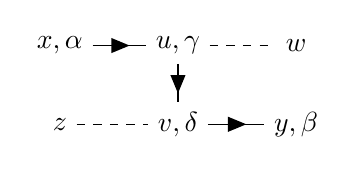
\begin{tikzpicture}
    \centering
\begin{feynman}
  \vertex (v0) at (-3.5, 0.5) {$x,\alpha$};
  \vertex[] (v1) at (-2, 0.5) {$u,\gamma$};
  \vertex[] (v2) at (-2, -0.5) {$v,\delta$};
  \vertex (v3) at (-0.5, -0.5) {$y,\beta$};
  \vertex (v4) at (-0.5, 0.5) {$w$};
  \vertex (v5) at (-3.5, -0.5) {$z$};
  \diagram* {
    (v0) -- [fermion] (v1),
    (v1) -- [fermion] (v2),
    (v2) -- [fermion] (v3),
    (v1) -- [scalar] (v4),
    (v5) -- [scalar] (v2)
  };
\end{feynman}
\end{tikzpicture}

Using Feynman's rules, this propagator is
\[
    G^{(4)}_{\psi_\alpha\bar\psi_\beta\phi\phi} = 
    (-ig)^2\int_{}^{} \dd^4v\dd^4u \Delta_{wu}\Delta_{zw}\delta_{\gamma\alpha}
    \delta_{\delta\beta}\left(
        S_{\alpha\gamma}(u-x)S_{\gamma\delta}(v-u)S_{\beta\delta}(y-v)
    \right)
\]

\textbf{Note} From the first order in $g$, Feynman rules can be deduced for any
theory and it is not necessary to compute $W$ to higher orders of $g$.

Plugging the F.Ts of the propagators into Green functions yields
\textit{the F.T. of Green functions}: these can be constructed by a different
set of Feynman rules 

The Feynman rules in momentum space are
\begin{itemize}
    \item To each line corresponds a $4-$momentum $k$: a free line
        yields a factor $1$, while a scalar propagator corresponds to a factor 
        \[
            \frac{i}{k^2-m^2+i\varepsilon}
        \]
    \item A fermionic propagator corresponds to
        \[
            i\frac{\slashed{k}+m}{k^2-m^2+i\varepsilon}
        \]
    \item An interaction point corresponds to
        \[
            -ig(2\pi)^4\delta_{\alpha\beta}\delta^4\left(\sum_{}^{}k_\text{in}
            -\sum_{}^{}k_\text{out}\right)
        \]
        where the $k$'s are taken with their sign and $\alpha,\beta$ are the
        spinor indices of the fermionic fields of the vertex.
\end{itemize}



\lesson{19/11}
\section{Scattering amplitudes}
The powerful part of QFTs is their predictions of scattering amplitudes
\[
    A=\bra{\text{out}}\ket{\text{in}}
\]
where ``out'' and ``in'' are the final and initial state of a system.

These quantities are obviously interesting in \textit{interacting theories}:
the interacting picture is more complicated than the free picture (as seen in
the IQFT course).

\subsection{Free theory}
The scalar fields of free theory can be expanded as
\[
    \phi(x)=\int_{}^{} \frac{\dd^3p}{(2\pi)^3\sqrt{2E_p}}e^{i\mathbf{p\cdot x}}
    \left(a(t,p)+a^\dagger(t,-p)\right):
\]
consider $t=0$
\[
    \ket{\text{f}}=\int_{}^{} \dd^3x f(0,\mathbf{x})\phi(0,\mathbf{x})\ket{0}=
    \int_{}^{} \dd^3x f(0,\mathbf{x})\int\frac{\dd^3p}{(2\pi)^3\sqrt{2E_p}}e^{i
    \mathbf{p\cdot x}}a^\dagger(0,-p)\ket{0}:=\int_{}^{} \frac{\dd^3p}{2E_p}
    \tilde f(\mathbf{p})\ket{\mathbf{p}}
\]
where
\begin{gather*}
    \ket{\mathbf{p}}:=\sqrt{2E_p}a^\dagger(0,\mathbf{-p})\ket{0},\\
    \tilde f(\mathbf{p})=\int_{}^{} \frac{\dd^3x}{(2\pi)^{\frac{3}{2}}}f(
    \mathbf{x})e^{i\mathbf{p\cdot x}}.
\end{gather*}
$f$ and $\tilde f$ can be set to create a ``wave packet'' of Gaussian form:
\[
    \tilde f(0,\mathbf{p})=\sigma^{-\frac{3}{4}}e^{-\frac{(\mathbf{p-k})^2}{2
    \sigma}}
\]
its anti-transform is
\[
    f(0,\mathbf{x})=\sigma^{\frac{3}{4}}e^{-\frac{x^2\sigma}{2}}e^{i\mathbf{k\cdot
    x}}.
\]
To compute their time evolution the Schrödinger picture is used:
\begin{gather*}
    i\pdv[]{}{t}\ket{t,f} = H\ket{t,f}\\
    \int_{}^{}\frac{\dd^3p}{2E_p}\pdv[]{\tilde f}{t}\ket{\mathbf{p}} =
    \int\frac{\dd^3p}{2E_p}\tilde f(t,\mathbf{p})\underbrace{H\ket{p}}_{
    =E_p\ket{\mathbf{p}}}\\
    i\pdv[]{\tilde f}{t} = E_p\tilde f(t,\mathbf{p} )
\end{gather*}
Imposing the initial condition stated before yields
\[
    \tilde f(t,\mathbf{p})=\sigma^{-\frac{3}{4}}e^{-\frac{(\mathbf{p-k})^2}{2
    \sigma}}e^{-iE_pt}
\]
The value of $E_p$ can be expanded around the value $p=k$, \textit{assuming}
$\sigma$ \textit{to be small},
\[
    E_p = E_k + \underbrace{\eval{\pdv[]{E_p}{p_i}}_{p=k}}_{:=v_k}(p_i-k_i)+...
\]
Plugging this in the exponent
\begin{gather*}
    f(t,\mathbf{x}) = \frac{1}{\sigma^{\frac{3}{4}}}\int \frac{\dd^3q}{2E_k}
    \exp\left[ -\frac{q^2}{2\sigma}-i\mathbf{v_k\cdot q}t - i\mathbf{q\cdot x}
    \right] \exp\left[ -iE_kt - i\mathbf{k\cdot x} \right]+...=\\=
    \frac{1}{\sigma^{\frac{3}{4}}} \int_{}^{} \frac{\dd^3q}{2E_k}
    \exp\left[ -\frac{1}{2\sigma}\left(\mathbf{q} + i\sigma(\mathbf{v_k}t+
    \mathbf{x})\right)^2 \right]+...
\end{gather*}
this is a simple Gaussian integral and yields\footnote{OCCHIO SEGNO DI X IN EXP}
\[
    f(t,\mathbf{x})=\sigma^{\frac{3}{4}}\frac{1}{2E_k}\exp\left[-\frac{\sigma}{2}
    \left(\mathbf{v_k}t-\mathbf{x}\right)^2 - iE_kt-i\mathbf{k\cdot x}\right]
\]
so this Gaussian is \textit{centred around its classical trajectory $x=v_kt$}.

For multi-particle states the form is similar:
\[
    \ket{f_1...f_n}=\int\prod_{i=1}^{n}\frac{\dd^3p_i}{2E_{p_i}}\tilde
    f_i(0,\mathbf{p_i}) \ket{\mathbf{p_1...p_n}}.
\]
The anti-transform at $t=0$ is the same as before for each particle:
\[
    f_i(0,\mathbf{x_i})=\sigma^{\frac{3}{4}}e^{-\frac{x_i^2\sigma}{2}}
    e^{i\mathbf{k_i\cdot x_i}}.
\]
And, unsurprisingly, also the time evolutions are the same
\begin{gather*}
    \tilde f_i(t,\mathbf{p_i})=\sigma^{-\frac{3}{4}}e^{-\frac{(\mathbf{p_i-k_i}
    )^2}{2\sigma}}e^{-iE_{p_i}t}\\
    f_i(t,\mathbf{x_i})=\sigma^{\frac{3}{4}}\frac{1}{2E_{k_i}}\exp\left[-\frac{
    \sigma}{2}\left(\mathbf{v_{k_i}}t-\mathbf{x_i}\right)^2 -
    iE_{k_i}t-i\mathbf{k_i\cdot x_i}\right]
\end{gather*}

\subsection{Interacting theory}
The fundamental assumption is that there exist a vacuum state ``close'' to the
free vacuum and that there exist a single particle state of momentum $\mathbf{p}$:
\[
    \ket{\mathbf{p}}\text{ with mass }m_p\sim m
\]
where $m$ is the bare mass (in AQFT it will be seen how $m$ and $m_p$ differ);
it is reasonable to assume this is an eigenstate of $H$ and of the momentum.

With this single particle state one can compute the quantities found before:
\begin{gather*}
    \ket{f} = \int_{}^{} \frac{\dd^3p}{2E_p}\tilde f(p)\ket{\mathbf{p}}\\
    \ket{t,f} = \frac{}{}\frac{\dd^3p}{2E_p}\tilde f(t,p)\ket{\mathbf{p}},
\end{gather*}
where $E_p = \sqrt{p^2-m_p^2}$.
To consider multiple particle states, one can assume that at $t=0$ they
are all in $x=0$, \textbf{but in the ``far'' past and future they do not interact,
therefore are free particle states}: this is the fundamental assumption
to consider scattering processes.

At $t=-\infty$ there is a state
\[
    \ket{\text{in}} = \int\prod_{i=1}^{n}\frac{\dd^3p_i}{2E_{p_i}}
    \tilde f_i(t,p_i)\ket{p_1...p_n}_\text{in}
\]
and similarly at $t=+\infty$
\[
    \ket{\text{out}} = \int\prod_{i=1}^{n}\frac{\dd^3p_i}{2E_{p_i}}
    \tilde f_i(t,p_i)\ket{p_1...p_n}_\text{out}.
\]

The free field
\[
    \phi(t,\mathbf{x}) = \int\dd^3p\left(g_p(t,x)a(p)+g^*_p(t,x)a^\dagger(p)
    \right) 
\]
where $g_p(t,x)$ can be found from the F.T. of the field.

It was shown in IQFT that
\begin{gather*}
    ia^\dagger (p)=\int_{}^{} \dd^3x g_p(t,x)\bar\pd_t\phi(t,x)\\
    -ia (p)=\int_{}^{} \dd^3x g^*_p(t,x)\bar\pd_t\phi(t,x)
\end{gather*}
where the derivatives act on both sides
\[
    g\bar\pd f = g\pd f - \pd g f.
\]
Their time derivatives are
\begin{gather*}
    i\pd_t a^\dagger (p) = \int_{}^{} \dd^3x\left(g_p(t,x)\ddot \phi - \ddot
    g_p(x,t)\phi\right) = \int_{}^{} \dd^3x \left(g_p(t,x)\ddot \phi - (
    \laplacian -m^2)g_p(t,x)\phi\right)
\end{gather*}
because $g_p$ satisfies the $K-G$ equation; this can be integrated by parts twice
to yield $(\Box +m^2) \phi=0$ in the free theory   
\[
    i\pd_ta^\dagger(p) = 0
\]
\section{LSZ reduction formula}
So in general these operators evolve in time, since for interacting fields the
$K-G$ equation is no longer homogeneous and the computed derivative does not
go to 0.
\begin{gather*}
    \lim\limits_{T\to-\infty} a^{(\dagger)}(t,p) = \sqrt{Z}a_\text{in}^{(\dagger)}
    (p)\\
    \lim\limits_{T\to+\infty} a^{(\dagger)}(t,p) =\sqrt{Z}a_\text{out}^{(\dagger)}
    (p)
\end{gather*}
[15 minuti]


\lesson{23/11}
So the quantities to be computed are probability amplitudes of the form
\[
    A=\phantom{x}_\text{out}\bra{q_1...q_m}\ket{p_1...p_n}_\text{in}
\]
where $p_i,q_j$ are momenta eigenstate.

For non-free theories it was found that
\[
    ia^\dagger(t,\mathbf{p})=\int\dd^3x g_p\bar{\pd_t} \phi(t,\mathbf{x})
\]
\[
    -ia(t,\mathbf{p})=\int\dd^3x g^*_p\bar{\pd_t} \phi(t,\mathbf{x})
\]
Their derivative was found to be
\[
    i\pd_ta^\dagger (t,\mathbf{p}) = \int_{}^{} \dd^3x g_p(\Box+m^2)\phi(t,
    \mathbf{x})
\]

A strategy to compute the amplitudes uses
\begin{gather*}
    \lim\limits_{T\to-\infty} a^{(\dagger)}(t,p) = \sqrt{Z}a_\text{in}^{(\dagger)}
    (p)\\
    \lim\limits_{T\to+\infty} a^{(\dagger)}(t,p) =\sqrt{Z}a_\text{out}^{(\dagger)}
    (p),
\end{gather*}
since
\[
    a_\text{in}^\dagger (\mathbf{p})\ket{0} = \sqrt{2E_p}\ket{p},
\]
the amplitude can be written as
\[
    \phantom{x}_\text{out}\bra{q_1...q_m}\frac{1}{\sqrt{2E_p}}a^\dagger_\text{in}
    (p_1)\ket{p_2...p_n}_\text{in}
\]
adding $0=a_\text{out}^\dagger(p_1)-a_\text{out}^\dagger(p_1)$ yields
\[
    \frac{1}{\sqrt{2E_p}}\phantom{x}_\text{out}\bra{q_1...q_m}a_\text{in}^\dagger
    -a_\text{out}^\dagger(p_1)\ket{p_2...p_n}_\text{in} +
    \frac{1}{\sqrt{2E_p}}\phantom{x}_\text{out}\bra{q_1...q_m}a^\dagger_\text{out}
    (p_1)\ket{p_2...p_n}_\text{in}.
\]
Assuming \textit{there is no forward scattering}, i.e. that no out particle has
the same momentum as any in particle (which means no particle remains
``untouched'' by the interaction), implies that the second addendum is zero (
since the $a^\dagger $ commutes with all bra creation operators that
create the out state and acts on the $\bra{0}$, yielding 0):
\[
    A = \frac{1}{\sqrt{2E_p}}\frac{-1}{\sqrt{Z}}\lim\limits_{T\to\infty}
    \phantom{x}_\text{out}
    \bra{q_1...q_m}
    \left(a^\dagger(T,p_1)-a^\dagger(-T,p_1)\right)\ket{p_2...p_n}_\text{in}
\]
The difference of the operators can be written as the integral over time of their
derivative
\begin{gather*}
    A = \frac{1}{\sqrt{2E_p}}\frac{-1}{\sqrt{Z}}\int_{-\infty}^{\infty} \dd t
    \phantom{x}_
    \text{out}\bra{q_1...q_m}\pd_ta^\dagger(t,p_1)\ket{p_2...p_n}_\text{in}=\\
    =\frac{1}{\sqrt{2E_p}}\frac{i}{\sqrt{Z}}\int_{}^{} \dd^4x_1g_{p_1}(x_1)
    (\Box_1+m^2)\phantom{x}_\text{out}\bra{q_1...q_m}\phi(x_1)\ket{p_2...p_n}_
    \text{in}
\end{gather*}
This process can be iterated to express $A$ in terms of the vacuum expectation
value of time ordered products of fields: one can 
express
\[
    \ket{p_2...p_n}_\text{in} = a^\dagger_\text{in}(p_2)\ket{p_3...p_n}
\]
and add
\[
    0=\left(a^\dagger_\text{out}(p_2)-a^\dagger_\text{out}(p_2)\right)\phi(x_1)
\]
and repeat the same process as before:
\[
    -\frac{1}{\sqrt{Z}}\lim\limits_{t_2\to\infty}\bra{q_1...q_m}a^\dagger(
    t_2,p_2)\phi(x_1)-a^\dagger(-t_2,p_2)\phi(x_1)\ket{p_3...p_n}\propto
    \int_{-\infty}^{\infty} \dd t_2 \pd_{t_2}\bra{q_1...q_m}T(a^\dagger(t_2,p_2)
    \phi(x_1)\ket{p_3...p_n}
\]  
and expressing $\pd_{t_2}a^\dagger(t_2,p_2)$ yields a term
\[
    \bra{q_1...q_m}T(\phi(x_2)\phi(x_1))\ket{p_3...p_n}.
\]
A similar strategy can be used to express $\bra{q_1...q_m}$ using $a$'s instead of
$a^\dagger$'s: after removing the initial states
\[
    \bra{q_1...q_m}T(\phi(x_1)...\phi(x_n))\ket{0} = 
    \bra{q_2...q_m}a_\text{out}(q_2)T(\phi_1...\phi_n) + T(...)(a_\text{in}(q_2)-
    a_\text{in}(q_2))\ket{0}
\]
from here, one can take the total time derivative, integrated over all time.

The final formula is
\begin{gather*}
A = \phantom{x}_\text{out}\bra{q_1..q_m}\ket{p_1..p_n}_\text{in}=\\=
\frac{i^n(-i)^m}{Z^{\frac{1}{2}(n+m)}}\int \left(\prod_{i=1}^{n} \dd^4x_i
\right)\left(\prod_{j=1}^{m}\dd^4y_j\right)\left(\prod_{i=1}^{n}\frac{g_{p_i}
(x_i)}{\sqrt{2E_{p_i}}}\right)\left(\prod_{j=1}^{m}\frac{g^*_{q_j}
(y_j)}{\sqrt{2E_{q_j}}}\right)(\Box_{x_1}+m^2)...(\Box_{x_n}+m^2)\\
(\Box_{y_1}+m^2)...(\Box_{y_m}+m^2)\bra{\Omega}T(\phi(y_1)...\phi(y_m)\phi(x_1)
...\phi(x_n))\ket{\Omega}.
\end{gather*}
The $g_p^{(*)}$ are plane waves and $x_i,y_j$ are integrated upon: these are
nothing but \textit{Fourier Transforms}.

The $\Box_{i}$'s become $-p_i^2$'s in momentum space:
\[
    A = \mathcal{N}\int\left(\prod_{i=1}^{n}\frac{\dd^4x_i}{(2\pi)^{\frac{3}{2}}}
    e^{ip_ix_i}\right)\left(\prod_{j=1}^{m}\frac{\dd^4y_j}{(2\pi)^{\frac{3}{2}}}
    e^{-iq_jy_j}\right)(-p_1^2+m^2)...(-q^2_m+m^2)\bra{\Omega}T(\phi_1...\phi_n...
    \phi_m)\ket{\Omega}
\]
\textbf{Note}: the particles are on shell, so the $(-p^2_k+m^2)$ should be all
zeroes, \textbf{but} the propagator has poles in the same points, so the
integrand is \textit{the amputated propagator}, since the poles 
associated to the external legs are simplified.

So at the end, the probability amplitude is
\textbf{the Fourier transform of the amputated propagator}:
\[
    A = \frac{i^n(-i)^m}{Z^{(n+m)/2}}\tilde{G}^\text{amp}(p_1...p_n;q_1...q_m)
    (2\pi)^4\delta^4\left(\sum p_i+\sum_{}^{}q_j\right)
\]

In principle, particles can be different and have different masses: they yield
different $Z$ factors, different mass terms  
\[
    A = \mathcal{N}\int\left(\prod_{i=1}^{n}\frac{\dd^4x_i}{(2\pi)^{\frac{3}{2}}}
    e^{ip_ix_i}\right)\left(\prod_{j=1}^{m}\frac{\dd^4y_j}{(2\pi)^{\frac{3}{2}}}
    e^{-iq_jy_j}\right)(-p_1^2+m_1^2)...(-q^2_m+m_m^2)\bra{\Omega}
    T(\phi_1(x_1)...\phi_n(x_n)...\phi_m(y_m))\ket{\Omega}
\]
where
\[
    \mathcal{N} = \frac{i^n(-i)^m}{\prod_{ij}Z_i^mZ_j^n}
\]
and $\phi_1...\phi_n...\phi_m$ are the $n+m$ different fields associated to the
$n+m$ different particles.
\subsection{Examples}
Let $\ket{in} = \ket{p_1,p_2}$ and $\ket{out} = \ket{q_1,q_2}$ in the
$\phi^4$ theory: there are two particles in and two particles out, so
the order is $\Lambda^2$ and there are 3 possible diagrams (since the
hypotesis of no forward scattering implies only connected diagrams):\\
\begin{tikzpicture}
\begin{feynman}
  \draw [scalar] (4, 0.5) arc [start angle=90, delta angle=180, radius=1];
  \draw [scalar] (4, 0.5) arc [start angle=90, delta angle=-180, radius=1];
  \vertex (v0) at (-2.5, 0.5) {};
  \vertex[dot] (v1) at (-1.5, -0.5) {};
  \vertex (v2) at (-2.5, -1.5) {};
  \vertex[dot] (v3) at (0.5, -0.5) {};
  \vertex (v4) at (1.5, 0.5) {};
  \vertex (v5) at (1.5, -1.5) {};
  \vertex (v6) at (2.5, 0.5) {};
  \vertex (v7) at (5.5, 0.5) {};
  \vertex (v8) at (2.5, -1.5) {};
  \vertex (v9) at (5.5, -1.5) {};
  \vertex[dot] (v10) at (4, 0.5) {};
  \vertex[dot] (v11) at (4, -1.5) {};
  \vertex (v12) at (6.5, 0.5) {};
  \vertex[empty dot, minimum size=0.025mm] (v13) at (8.5, 0.5) {};
  \vertex (v14) at (6.5, -1.5) {};
  \vertex[empty dot, minimum size=0.1mm] (v15) at (8.5, -1.5) {};
  \vertex[dot] (v16) at (7.5, 0.5) {};
  \vertex[dot] (v17) at (7.5, -1.5) {};
  \vertex (v18) at (10.5, -1.5) {};
  \vertex (v19) at (10.5, 0.5) {};
  \diagram* {
    (v0) -- [scalar] (v1),
    (v1) -- [scalar] (v2),
    (v1) -- [scalar, bend right=45] (v3),
    (v1) -- [scalar, bend left=45] (v3),
    (v3) -- [scalar] (v4),
    (v3) -- [scalar] (v5),
    (v6) -- [scalar] (v7),
    (v8) -- [scalar] (v9),
    (v12) -- [scalar] (v13),
    (v14) -- [scalar] (v15),
    (v16) -- [scalar, bend right=45] (v17),
    (v16) -- [scalar, bend left=45] (v17),
    (v15) -- [scalar] (v19)
  };
  \begin{scope}[even odd rule]
    \clip (-5, -4) rectangle (13, 3) (9.5, -0.5) circle (0.082cm);
    \path (v13) edge [scalar] (v18);
  \end{scope}
\end{feynman}
\end{tikzpicture}



Using Feynman rules the propagator can be computed as the sum of $3$ propagators



\end{document}
